\label{sec:impedances}

The cooling path between the sources dissipating electrical power and the cooling fluid is 3-dimensional and includes components with orthotropic thermal conductivity. Hence the prediction of temperature at any node of the model requires a 3D thermal FEA \cite{abaqus,ansys}. However, the thermal conductivities of the components along the path are approximately constant, so that the temperature rise $\Delta T_i$ above the coolant temperature of any node $i$ ($i=$~ABC, HCC, AMAC, FEAST, tape, RHV, or sensor) in the thermal network model is adequately described by a linear sum of contributions from individual sources, i.e:

\begin{equation}
\Delta T_i \equiv T_i - T_C = R_i P_i + \left(R_\text{C} + R_\text{M}\right)\sum_j P_j,
\label{eq:deltaT_expression}
\end{equation}
where the index $j$ runs over all powered nodes. (We have momentarily ignored the contribution from the EOS card.)

In order to extract the thermal impedances for the thermal network model, the finite element model is run multiple times, with each heat source (or group of similar sources) switched on in turn with a representative amount of heat. In each of these cases, the temperature is calculated for all nodes in the thermal network model (Fig.~\ref{fig:thermalmodel}). The temperature of a node is here taken as the average of the temperatures for all the grid points in the FEA model within the volume of the object corresponding to the node\footnote{This is particularly interesting in the case of the sensor, which fills a large volume, with a potentially large range of temperatures. In Ref.~\cite{Beck:2010zzd} the analytic model parameters were extracted from the maximum sensor temperature predicted by FEA, whereas our subsequent studies have shown that the thermal stability limit is predicted more accurately if the average sensor temperature is used.}. The thermal impedances are then obtained from a fit of Eq.~\ref{eq:deltaT_expression} using the temperature data for all nodes for all cases of heat injection.

Because of the nature of the network, the fitted value for the common impedance $R_\text{CM}=R_\text{C} + R_\text{M}$ is determined by the observed temperature rises of components where no heat is injected. The linearity of this relationship is illustrated in Fig.~\ref{fig:solving_for_Rcm}. The value of each component-specific impedance is determined from the temperature rise observed when heat is injected into that component. The linear approximation of the model reasonably describes the FEA simulation, and the level of disagreement, discussed below, is taken as an uncertainty that is assessed as a safety factor as described in Section~\ref{sec:safety_factors}.

%The cooling path between the sources dissipating electrical power and the cooling fluid is three-dimensional and includes components with orthotropic thermal conductivity. Hence the prediction of temperature at any node of the model requires a 3d thermal FEA Ref [Abaqus, Ansys]. However, the thermal conductivities of the components along the path are approximately constant, so that the temperature rise (above Tc) at any node of the structure is adequately described by a linear sum of contributions from individual sources, i.e:
%\begin{equation}
%T_i  =   T_\text{c}  +  \sum_{j} a_{ij} Q_{j},
%\end{equation}

%(or group of similar sources) switched on in turn with a representative amount of heat, and the temperature rise noted for each of the nodes of interest, which are those in the thermal network model (Fig.~\ref{fig:thermalmodel}).  

%BEGIN ALTERNATE DESCRIPTION
%Ignoring the EOS components momentarily, the temperature rise $\Delta T_i \equiv T_i - T_c$ of a given node $i$ can be expressed as:
%\begin{equation}
%\Delta T_i = R_i P_i + \left(R_{C} + R_{M}\right)\sum_j P_j\,, \quad i,j=(\text{ABC},\text{HCC},\text{AMAC},\text{FEAST},\text{tape},\text{RHV},\text{sensor}),/
%\label{eq:deltaT_expression}
%\end{equation}
%where the powered components are represented by the index $j$.
%In order to extract the coefficients $R_{i}$, $R_{C}$ and $R_{M}$,
%the finite element model is run multiple times, with each heat source (or group of similar sources)
%switched on in turn with a representative amount of heat, and the temperature rise
%noted for each of the nodes of interest, which are those in the thermal network model (Fig.~\ref{fig:thermalmodel}).
%
%Using this data from the FEA, the quantity $R_{CM}\equiv R_{C} + R_{M}$ is first solved by
%focusing on the set of measurements where the measured temperature node ($i$)
%is not associated to the powered component ($j$).
%In these cases, the relationship can be expressed as:
%\begin{equation}
%\Delta T_i = R_{CM} P_j,
%\end{equation}
%assuming that only one source $j$ is powered at a time.
%Each pair of values for delivered power and $\Delta T$ is plotted in Fig.~\ref{fig:solving_for_Rcm}.
%The data is fit to a function of the form $\Delta T = R_{CM} \times P$;
%the slope of the line corresponds to the thermal impedance $R_{CM}$.
%The remaining thermal impedances ($R_\text{FEAST}$, $R_\text{ABC}$, etc.) are calculated by
%subsituting $R_{CM}$ into the equations remaining from Eq.~\ref{eq:deltaT_expression}.
%The value $R_{EOS}$ is calculated using a simlar procedure.

\begin{figure}[ht]
\centering
\subfloat[Barrel short strip module] {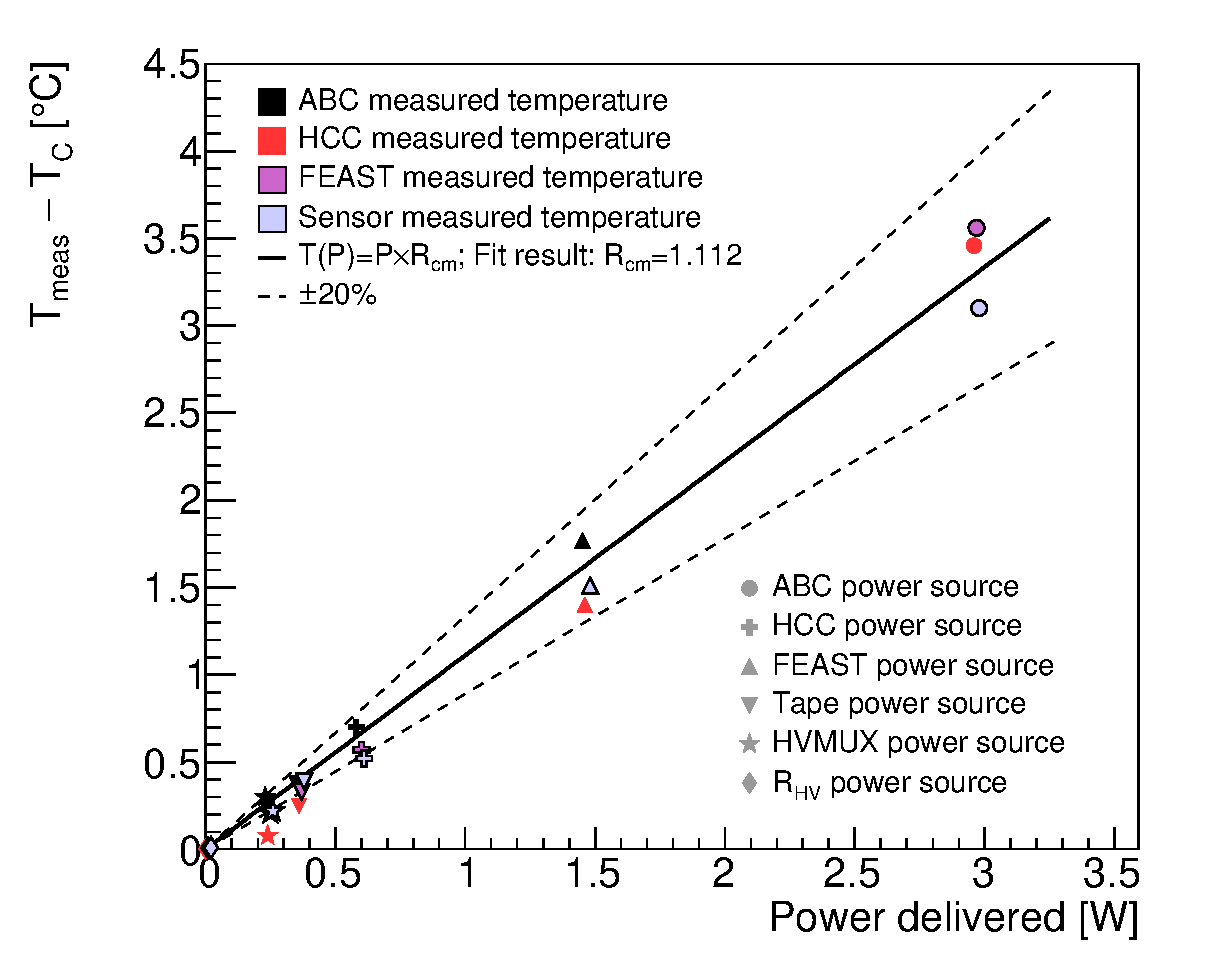
\includegraphics[width=0.45\linewidth]{figures/ThermalImpedanceFit_ShortStripEOS_Rcm.eps}}\quad\quad
\subfloat[Endcap R0 module] {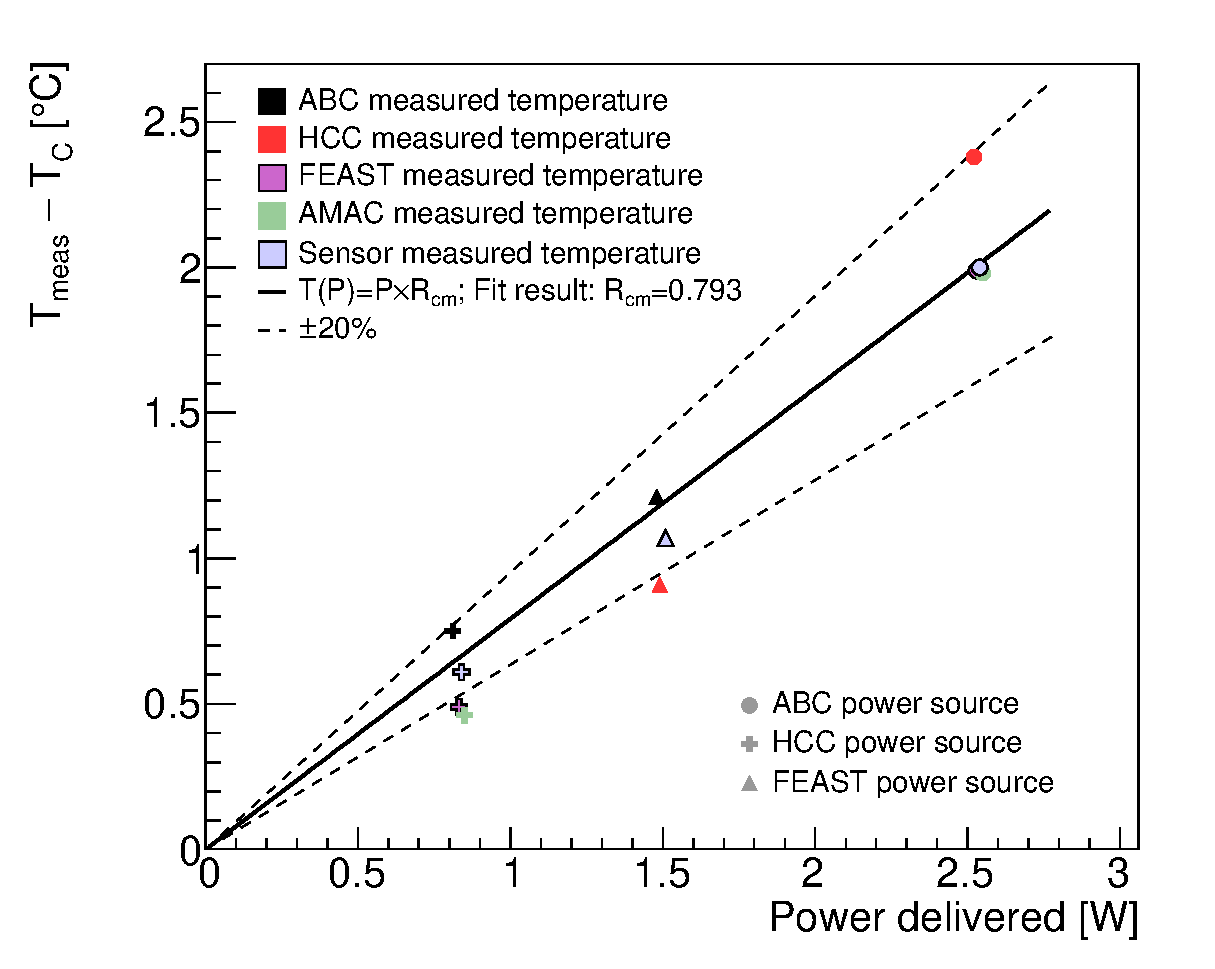
\includegraphics[width=0.45\linewidth]{figures/ThermalImpedanceFit_R0_Rcm.eps}}
\caption{The relationship between the temperature rise observed in the FEA for a specific component and the heat injected in another component. The slope of the fitted line is the estimate for $R_\text{CM}$.
(a) The fit for a short-strip barrel module adjacent to the EOS card. (b) The fit for the endcap R0 module.
For each data point marker, the source of power is indicated by the shape, and the measured component is indicated
by the colour (black: ABC, red: HCC, magenta: FEAST, green: AMAC, light blue: silicon sensor).
%% In (b), the error bars represent the standard deviation of temperatures of
%% that particular component, and are not considered in the fit.
The dashed lines represent a $\pm$20\% error band on the fit for $R_\text{CM}$.
}
\label{fig:solving_for_Rcm}
\end{figure}

%END ALTERNATE DESCRIPTION

For a barrel module, the agreement of the network temperatures using the thermal impedances from the fit with the data from FEA is better than 0.5$^\circ$C for all nodes. This procedure is performed for both an EOS module and a normal module. The thermal impedance from the sensor to the sink ($R_\text{CM}$) is consistently between 1.1 and 1.4~$^\circ$C/W, but higher values (between 10 and 20~$^\circ$C/W) are found for other impedances in the network ($R_\text{HCC}$ and $R_\text{FEAST}$), mostly because these are for components with a small footprint constituting a bottleneck for the heat flow.
A 10\% uncertainty is assigned to the thermal impedances in the barrel modules for the purposes of assessing safety factors.

% Endcap: 
For the endcap modules, the procedure to determine the thermal impedances is performed for
each of the 6 module types. $R_\text{CM}$ ranges from 0.6 to 1.4~$^\circ$C/W, with other nodes
between 5 and 20~$^\circ$C/W. Because the location of powered components is more irregular on an
endcap module, the difference between the predicted temperatures of the linear network and the FEA
can reach up to 1.2~$^\circ$C for key temperature-dependent nodes. Therefore, a 20\% uncertainty is assigned
to the thermal impedances in the endcap modules.

There are two recognised departures from linearity of the thermal path: the rise in thermal conductivity of the silicon sensor with decreasing temperature, and the rise in heat transfer coefficient (HTC) of the evaporating CO$_2$ coolant with increasing thermal flux. The FEA models are run using mean values for these quantities appropriate to the operating conditions, and the thermo-electrical model results are insensitive to the variations expected in practice. However, if this level of realism is required and if reliable parametrizations for these dependencies can be obtained, then the inclusion of such variations in the model is possible.
